\documentclass[tikz,border=10pt]{standalone}
\usepackage{amsmath}
\pagecolor[HTML]{171D2B}
\definecolor{aksen}{HTML}{F7B538}
\begin{document}
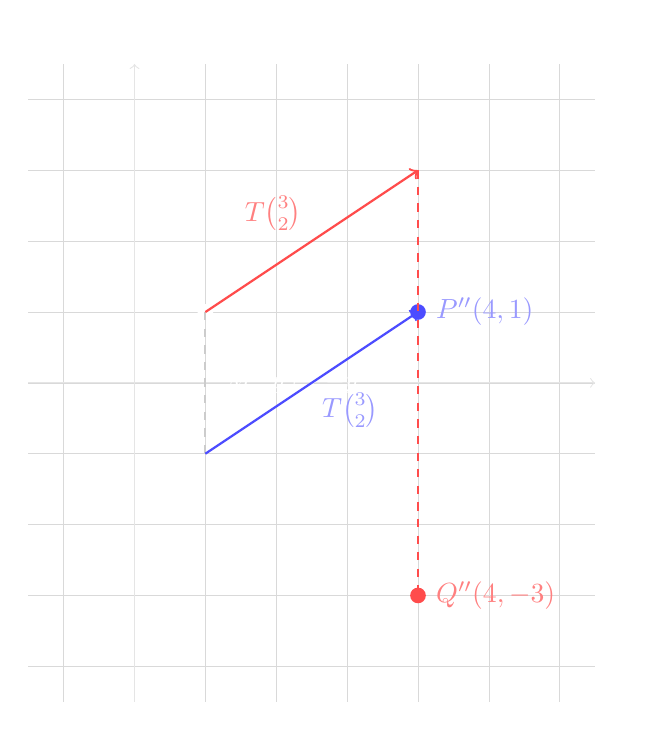
\begin{tikzpicture}[scale=0.9,
    titik/.style={circle, fill=white, inner sep=2pt},
    lab/.style={text=white, font=\small}]
  % grid & sumbu
  \draw[gray!30, very thin] (-1.5,-4.5) grid (6.5,4.5);
  \draw[white!80!gray, ->] (-1.5,0) -- (6.5,0) node[right, text=white] {$x$};
  \draw[white!80!gray, ->] (0,-4.5) -- (0,4.5) node[above, text=white] {$y$};
  % titik awal
  \node[titik, label={[lab]above left:$P(1,1)$}] at (1,1) {};
  % jalur A: refleksi dulu (garis putus), lalu translasi (biru)
  \draw[dashed, thick, white!60!gray] (1,1) -- (1,-1);
  \node[lab, right] at (1.15,0) {$M$: $y \mapsto -y$};
  \draw[->, thick, blue!70] (1,-1) -- (4,1)
        node[midway, below right, text=blue!40] {$T\binom{3}{2}$};
  \node[titik, fill=blue!70, label={[text=blue!40]right:$P''(4,1)$}] at (4,1) {};
  % jalur B: translasi dulu (merah), lalu refleksi (garis putus)
  \draw[->, thick, red!70] (1,1) -- (4,3)
        node[midway, above left, text=red!50] {$T\binom{3}{2}$};
  \draw[dashed, thick, red!70] (4,3) -- (4,-3);
  \node[titik, fill=red!70, label={[text=red!50]right:$Q''(4,-3)$}] at (4,-3) {};
\end{tikzpicture}
\end{document}
